\section{Literature Review} \label{sec:lit-review}

\subsection{QTL mapping and MAS}

The wide availability and reduced cost of molecular marker technology
has created opportunities to perform marker assisted selection of genotypes
in plant and animal breeding. Quantitative Trait Locus (QTL) mapping techniques
have proved useful for detecting the effects of small numbers of markers producing 
phenotypes with large effects \citep{miles2008}. Once a sufficient proportion of
critical QTL markers have been identified, they can be leveraged for making selections
on a population. Using identified QTL to support selection has grown in popularity
as molecular marker data costs have decreased. Individuals in a population
can be genotyped for previously identified QTL markers are subsequently selected 
upon based on the presence of desired alleles and/or haplotypes.
When only select genetic markers are used to select for a quantitative trait,
this process is known as Marker Assisted Selection (MAS). MAS is usually effective on
traits with a few large effect alleles with high heritability. However, when making selections 
on traits with many contributing small effect alleles distributed widely 
across a genome, MAS becomes less effective \citep{heffner2009}. 

In order to leverage MAS for traits with diverse genetic architectures, is is
advisable to combine MAS on juvenile individuals and subsequent phenotypic
selection on adults with favorable MAS scores \citep{lande1990}. This process, 
known as two-stage selection, proved effective for improving
the coefficient of selection of breeding programs while avoiding expensive phenotypic
trials for individuals with low genetic potential. While inexpensive, two-stage selection 
only utilizes select markers with significant QTL effects. The present cost of
genome wide SNP assays has fallen dramatically enough that today individuals are
frequently genotyped for hundreds, thousands, or even tens of thousands of SNPs. 
Information in SNPs that are not significantly associated with a trait are lost 
when applying MAS and two-stage selection, but could provide improved predictive 
accuracy on individual's genetic value.

\subsection{Genomic Prediction}

Unlike QTL mapping and associated MAS techniques, genomic prediction methods 
attempt to predict phenotypes utilizing all available SNP marker data collected 
from a population, allowing one of many possible statistical models to learn 
the marker-trait associations in a data driven way \citep{meuwissen2001}. 
The accuracy of genomic prediction relies on an appropriate choice of statistical model that 
will capture the relationship between the genetic architecture
of a trait and the underlying marker calls in a panel of high-density marker 
data. It is likely that the best statistical model for genomic prediction is 
dependent on the genetic architecture of 
the predicted trait \citep{crossa2010, gonzalez-camacho2012, 
resende2012, cleveland2012, thavamanikumar2015}.  From a mathematical perspective,
models incorporating interactions between marker features have the 
capacity to achieve higher accuracy by capturing non-additive effects. 
Experimental results support this hypothesis \citep{gonzalez-camacho2012}. 
Alternative prediction methods continue to be an active area of research 
in plant and animal breeding \citep{koning2012}.

Once an accurate and predictive model of a QTL is discovered and a SNP marker
assay has been conducted on an individual, it is trivial to convert the underlying
predictions into a selection index. If the predictive model is selected 
such that it captures only additive effects, the resulting predictions can be 
considered to be an estimate of the breeding value of the assayed individual.
To differentiate breeding values estimated from genomic panels from breeding values
calculated via traditional phenotypic measurements and best linear unbiased prediction (BLUP)
models, the term genome estimated breeding value or GEBV was coined \citep{meuwissen2002}.

\subsection{Choosing a Genomic Prediction Model}

Genomic prediction presents a distinct mathematical challenge compared to MAS.
When conducting MAS, a large number of individuals $n$ are evaluated at a
comparatively smaller number of loci $p$. In a general sense, this corresponds 
to solving an overdetermined system of linear equations. The large family of 
regresson techniques that minimize a least-squares loss function are well
behaved on overdetermined systems. Genomic prediction is characterized by the opposite
scenario where $n < p$. Typically a smaller number of individuals are genotyped
at a larger number of marker loci. These problems can be solved using least squares regression,
but also require that a regularization penalty is defined in addition to the least-squares 
loss function that is used to select between possible solutions to the underdetermined
system. 

There are many forms of regularization. Perhaps the best known regularization
method is L2 regularization, which penalizes overly large regression coefficients in least 
squares regression problems \citep{tibshirani1996}. L2 regularization prefers solutions that utilize all available 
input features to make a prediction rather than favoring only a few features. Ridge regression
is a L2 regularized ordinary least squares regression. The $\lambda$ parameter to
the ridge regression model adjusts the penalty applied to large coefficients. Another common
form of regularization is L1 regularization \citep{tibshirani1996}. L1 regularization penalizes the sum of the regression
coefficients in least squares regression problems. Where L2 regularization prefers solutions that
utilize all input features, L1 prefers solutions that set non-informative features coefficients
to zero. Least absolute shrinkage and selection operator (LASSO) regression is an L1 regularized
linear regression. These and other regularization techniques are described in the context
of neural network models in Subsection \ref{ssec:neuralnets}.

Different regularization techniques such as L1 and L2 regularization have a relationship
to the genetic architecture of the trait they are predicting. If a trait has many small 
effect markers, models incorporating L2 regularization are likely to perform better
than unregularized models. Classical MAS traits with small number of large effect
markers may be best predicted with by algorithms incorporating L1 regularization. 
Traits falling somewhere in between may do well with models incorporating a combination
of L1 and L2 regularization such as the so-called elastic net regression \citep{zou2005}.

A wide variety or regularization techinques exist. Some are broadly used and simple
to reason about like L1 and L2 regularization. Others are applicable only to certain 
classes of mathematical models such as assumed prior distributions in bayesian
regression methods. When attempting genomic prediction, it is critical to evaluate 
the available regularization techniques for multiple prediction methods ideally selecting 
a single model with zero or more regularization techniques in a data-driven way such 
as cross validation. 

\subsection{Data Science}

Concurrent with the advent of genomic prediction as a practice the popularity of the 
interdisciplinary field known as data science has increased. Practitioners of data 
science, known as data scientists, apply machine learning and statistics to make 
predictions, usually by applying ideas or techniques from a wide variety of domains 
including mathematics, statistics, and computer science. Often, a data scientist's focus is to
create a predictive model that may not be associated with an underlying generative model. 
Some view this as the distinction between data science and classical statistics 
\citep{donoho2015, breiman2001}. The rapid increase in popularity of data science
is associated with better definitions of best practices for predictive modeling
across many disciplines as well as software packages to automate the 
process of building predictive models from any data source.

Data scientists have used their experience to improve existing statistical 
models and tackle problems of immense complexity, some of which were previously 
thought unsolvable. Considering only applications of neural networks, data scientists
applied networks to recognize handwritten text, as well as identify spoken 
words in real-time audio recordings \citep{lang1990}.
Data scientists compared the performance of a neural networks model to a traditional 
logistic regression model used to detect signals indicating epilepsy in electroencephalograph 
readings and found the network unanimously outperformed the existing model \citep{subasi2005}.
A complex neural network archetecture learned to play seven different Atari 2600 
games using screen pixels as input and training the network to maximize the "score" of
the game it was trained on \citep{mnih2013}. These results demonstrate that data scientists
can employ machine learning to solve problems or improve predictive accuracy on large and 
complex datasets from a wide variety of technical fields.

The rise in successful outcomes from individuals employing data science
methodologies has renewed interest in the machine learning field in both
private and public sectors. Many universities are now offering advanced cross-disciplinary
degrees in data science that include statistics, mathematics, and computer
science courses. Genomic prediction is one of many opportunities for data scientists
to apply data science practices to plant and animal breeding.

\subsection{Popular Models}

Lorem Ipsum.

\subsection{Neural Network Architecture} \label{ssec:neuralnets}

Neural networks are a type of model frequently employed by data scientists
for predictive modeling. Neural networks consist of layers of interconnected neurons
which map inputs to one or more outputs. Each neuron in a network can be expressed as a 
transformation of a weighted sum of $n$ inputs 

\begin{equation}
output_{lk} = \sum_{i=1}^{n} f_l(w_{lki} * x_{i} + b_{lk})
\label{eq:neuron}
\end{equation}

where $output_{lk}$ is the output from neuron $k$ in network layer $l$ having activation
function $f_l$, weights $w_{lki}$ and bias $b_{lk}$.

A neural network is a collection of neurons that map a 
length $n$ input vector $x = (x_1, ..., x_n)$ through a series of $j$ 
"hidden" layers $(l_1, ..., l_j)$. Each hidden layer consists of a variable 
number of neurons, each of which apply an associated coefficient, bias, and 
mathematical transformation to their input and forward the 
result on to every neuron in the subsequent layer forming an interconnected 
network (Figure \ref{fig:simplenet}).

\ifdefined\showtablesandfigures
% A simple neuralnet with one hidden layer.

\begin{figure}[htbp]
\renewcommand{\familydefault}{\sfdefault}\normalfont
\centering

\def\layersep{2.0cm}

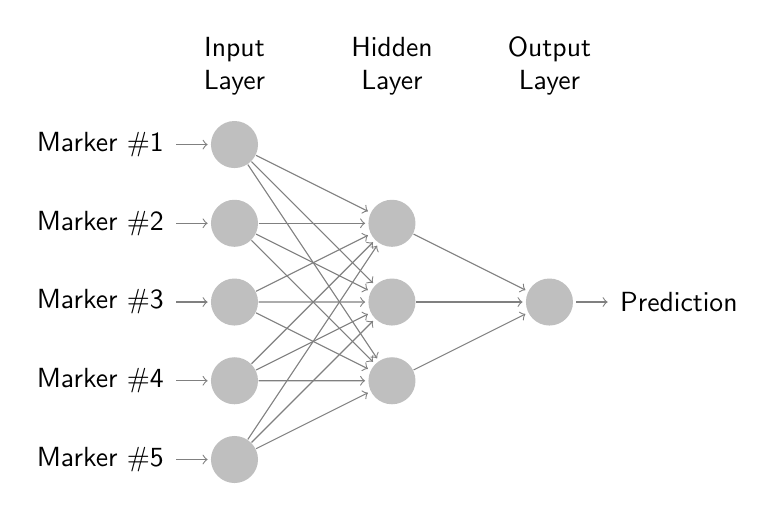
\begin{tikzpicture}[shorten >=1pt, ->, draw=black!50, node distance=\layersep]
    \tikzstyle{every pin edge}=[<-, shorten <=1pt]

    \tikzstyle{neuron}=[circle, fill=black!25,minimum size=17pt, inner sep=0pt]
    \tikzstyle{input neuron}=[neuron];
    \tikzstyle{output neuron}=[neuron];
    \tikzstyle{hidden neuron}=[neuron];

    \tikzstyle{annot}=[text width=4em, text centered]

    \foreach \name / \y in {1,...,5}
        \node[input neuron, pin=left:Marker \#\y] (I-\name) at (0,-\y) {};

    \foreach \name / \y in {1,...,3}
        \path[yshift=-1cm]
            node[hidden neuron] (H-\name) at (\layersep,-\y cm) {};

    \node[output neuron, pin={[pin edge={->}]right:Prediction}, right of=H-2] (0) {};

    \foreach \source in {1,...,5}
        \foreach \dest in {1,...,3}
            \path (I-\source) edge (H-\dest);

    \foreach \source in {1,...,3}
        \path (H-\source) edge (0);

    \node[annot, above of=I-1, node distance=1cm] (il) {Input Layer};
    \node[annot, right of=il] (hl) {Hidden Layer};
    \node[annot, right of=hl] {Output Layer};
\end{tikzpicture}

    \caption{A multi-layer perceptron neural network with a single hidden layer. 
             Many input calls are mapped into the hidden layer of neurons. For genomic
             prediction, the input layer consists of one neuron per marker and the output
             consists of a single neuron which combines the information from the final
             hidden layer to predict a phenotype or BLUP. Because this network has only
             a single hidden layer, it would not be considered a deep network.}

\label{fig:simplenet}
\end{figure}
 % Label = fig:simplenet
\fi


Once the network is defined, it must be exposed to input and desired output
values, and adjusted to minimize error in output in a process known as training.
The weights and biases are often initialized by drawing from a
random normal distribution. From this initial state, error in 
the output of the network is propagated back through the hidden 
layers, and the weights and biases are updated in the direction that would 
decrease output error on many sets or subsets of the input data. 
This turns the network training process into general 
function minimization problem, where the parameters to the function are the 
weights and biases of the network neurons and the function to be 
minimized is the squared differences between the network outputs and 
the desired true values. The process of propagating output error back 
through a neural network is known as backpropagation, and has been used 
and improved extensively since its original description in the 
1980s \citep{rumelhart1986}.  Typically, the training data is split 
evenly into representative, randomly sampled collections of data 
called batches. The training algorithm exposes the network to each 
batch until they are depleted, after which the process is repeated. Each 
collection of batches is known as an epoch, and training typically 
involves applying backpropagation for several hundred epochs, or until the network
weights and biases reach an equilibrium state that has converged to a 
globally minimum amount of prediction error.

%Good post, good links to the 'deep' part of deep nets.
%http://stats.stackexchange.com/questions/182734/what-is-the-difference-between-a-neural-network-and-a-deep-neural-network

It is trivial to add additional hidden layers to a neural network 
model once it has been defined (Compare Figure \ref{fig:simplenet} to Figure \ref{fig:deepnet}). 
Despite the ease of describing their architecture, networks with many hidden 
layers have been notoriously difficult to train due to
the vanishing gradient problem \citep{hochreiter1998}. Recently, a series 
of breakthroughs in neural network training as well as computer
hardware speed have allowed efficient training of deeper networks 
than were previously possible \citep{sutskever2013}.
A history of the deep learning literature is available in \cite{lecun2015}.
The increased training efficiency and potential to capture subtle
correlation relationships between two or more input features drove a need to 
differentiate these deeper networks from prior work, resulting in 
the emergence of the phrase "deep learning" to describe the construction 
and training of deep neural networks.

\subsection{Neural Networks for Genomic Prediction}

Attempts to apply neural networks to genomic prediction has resulted in overfitting of the 
network to training data as well as concerns over the 
computation time required to fit the model to datasets with many
markers across many genotypes \citep{heslot2012, gonzalez-recio2014}. 
These results are not surprising. Multi-layer feedforward neural networks 
are capable of approximating functions of arbitrary complexity to arbitrary 
accuracy if provided enough neurons in even a single hidden 
layer. This property of neural networks is known as the 
universal approximation theorem, and can result in 
overfitting if the weights of the network are not regularized in some way \citep{hornik1989}.

Given the promising results from regularized and bayesian methods for 
genomic prediction such as ridge or lasso regression and the bayesian family of regressors,
it is prudent to evaluate some of the many of neural network training algorithms which
incorporate regularization of weights during training. Today, networks based on these 
and other regularization techniques continue to achieve award-winning performance 
across many domains \citep{schmidhuber2015}. Similarly, while neural networks are 
computationally demanding to train, the training algorithms 
themselves are often easily expressed with vector and matrix algebra and thus amenable to
Graphics Processing Unit (GPU) accelerated computing. Some report up to sixty-fold speedups 
in training time \citep{sierra2010, schmidhuber2015}. 

In this paper, we present the results of applying deep neural networks
to genomic prediction. We explore two types of network regularization
to deep neural networks. The first is a weight decay regularization
which penalizes the weights $W$ with very large values 
similar to ridge regression \citep{krogh1992}. The second is dropout 
regularization, in which a portion of neurons and their connections are removed 
at random during each training epoch, encouraging subsets of the network to learn 
to recognize input features independently. This allows neurons to adapt 
and build independently operating units and prevents the 
neurons from co-adapting, reducing overfitting \citep{srivastava2014}.  
We also quantitatively evaluate the time required to train neural networks
using both CPU and GPU based network fitting. Last, we compare the 
performance of regularized networks with other competitive genomic prediction models.

% For the introduction, authors should be mindful of the broad readership of the journal. i
% The introduction should set the stage for the importance of the work to a generalist 
% reader and draw the reader in to the specific study. The scope and impact of the 
% work should be clearly stated.

\subsection{Genomic Selection in a Breeding Program}

Lorem ipsum.

